\documentclass{standalone}
\usepackage{tikz}
\usetikzlibrary{patterns, positioning}

\begin{document}
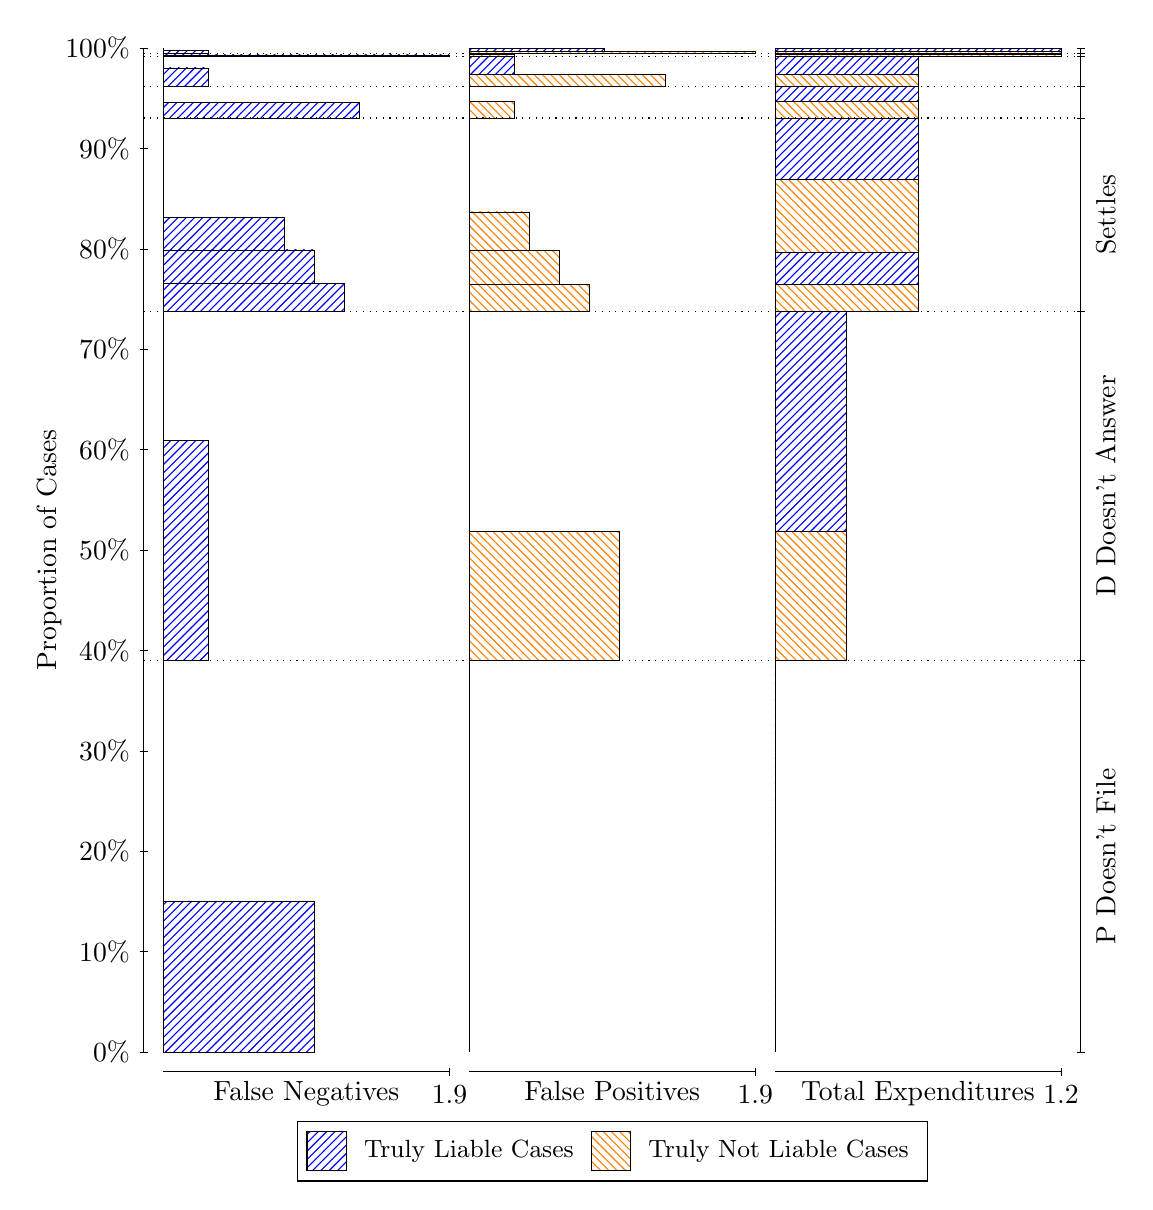
\begin{tikzpicture}
\draw[black, very thin] (1.5,1.75) -- (1.5,14.5);
\node[rotate=90, anchor=center] at (0.3, 8.125) {Proportion of Cases};
\draw[black, very thin] (1.45,1.75) -- (1.55,1.75);
\node[anchor=east] at (1.45, 1.75) {0\%};
\draw[black, very thin] (1.45,3.025) -- (1.55,3.025);
\node[anchor=east] at (1.45, 3.025) {10\%};
\draw[black, very thin] (1.45,4.3) -- (1.55,4.3);
\node[anchor=east] at (1.45, 4.3) {20\%};
\draw[black, very thin] (1.45,5.575) -- (1.55,5.575);
\node[anchor=east] at (1.45, 5.575) {30\%};
\draw[black, very thin] (1.45,6.85) -- (1.55,6.85);
\node[anchor=east] at (1.45, 6.85) {40\%};
\draw[black, very thin] (1.45,8.125) -- (1.55,8.125);
\node[anchor=east] at (1.45, 8.125) {50\%};
\draw[black, very thin] (1.45,9.4) -- (1.55,9.4);
\node[anchor=east] at (1.45, 9.4) {60\%};
\draw[black, very thin] (1.45,10.675) -- (1.55,10.675);
\node[anchor=east] at (1.45, 10.675) {70\%};
\draw[black, very thin] (1.45,11.95) -- (1.55,11.95);
\node[anchor=east] at (1.45, 11.95) {80\%};
\draw[black, very thin] (1.45,13.225) -- (1.55,13.225);
\node[anchor=east] at (1.45, 13.225) {90\%};
\draw[black, very thin] (1.45,14.5) -- (1.55,14.5);
\node[anchor=east] at (1.45, 14.5) {100\%};

\draw[black, very thin] (13.4,1.75) -- (13.4,14.5);
\draw[black, very thin] (13.35,1.75) -- (13.45,1.75);
\node[anchor=west] at (13.35, 1.75) {};
\draw[black, very thin] (13.35,6.7219) -- (13.45,6.7219);
\node[anchor=west] at (13.35, 6.7219) {};
\draw[black, very thin] (13.35,11.156) -- (13.45,11.156);
\node[anchor=west] at (13.35, 11.156) {};
\draw[black, very thin] (13.35,13.611) -- (13.45,13.611);
\node[anchor=west] at (13.35, 13.611) {};
\draw[black, very thin] (13.35,14.017) -- (13.45,14.017);
\node[anchor=west] at (13.35, 14.017) {};
\draw[black, very thin] (13.35,14.396) -- (13.45,14.396);
\node[anchor=west] at (13.35, 14.396) {};
\draw[black, very thin] (13.35,14.433) -- (13.45,14.433);
\node[anchor=west] at (13.35, 14.433) {};
\draw[black, very thin] (13.35,14.5) -- (13.45,14.5);
\node[anchor=west] at (13.35, 14.5) {};

\draw[black, very thin, pattern color=blue, pattern=north east lines] (1.75,1.75) rectangle (3.6623,3.6597);
\draw[black, very thin, pattern color=orange, pattern=north west lines] (1.75,3.6597) rectangle (1.75,6.7219);
\draw[black, very thin, pattern color=blue, pattern=north east lines] (1.75,6.7219) rectangle (2.3237,9.5154);
\draw[black, very thin, pattern color=orange, pattern=north west lines] (1.75,9.5154) rectangle (1.75,11.156);
\draw[black, very thin, pattern color=blue, pattern=north east lines] (1.75,11.156) rectangle (4.0447,11.515);
\draw[black, very thin, pattern color=blue, pattern=north east lines] (1.75,11.515) rectangle (3.6623,11.936);
\draw[black, very thin, pattern color=blue, pattern=north east lines] (1.75,11.936) rectangle (3.2798,12.347);
\draw[black, very thin, pattern color=orange, pattern=north west lines] (1.75,12.347) rectangle (1.75,13.611);
\draw[black, very thin, pattern color=blue, pattern=north east lines] (1.75,13.611) rectangle (4.236,13.805);
\draw[black, very thin, pattern color=orange, pattern=north west lines] (1.75,13.805) rectangle (1.75,14.017);
\draw[black, very thin, pattern color=blue, pattern=north east lines] (1.75,14.017) rectangle (2.3237,14.247);
\draw[black, very thin, pattern color=orange, pattern=north west lines] (1.75,14.247) rectangle (1.75,14.396);
\draw[black, very thin, pattern color=blue, pattern=north east lines] (1.75,14.396) rectangle (5.3833,14.414);
\draw[black, very thin, pattern color=orange, pattern=north west lines] (1.75,14.414) rectangle (1.75,14.433);
\draw[black, very thin, pattern color=blue, pattern=north east lines] (1.75,14.433) rectangle (2.3237,14.472);
\draw[black, very thin, pattern color=orange, pattern=north west lines] (1.75,14.472) rectangle (1.75,14.5);
\draw[black, very thin, pattern color=orange, pattern=north west lines] (5.6333,1.75) rectangle (5.6333,4.8121);
\draw[black, very thin, pattern color=blue, pattern=north east lines] (5.6333,4.8121) rectangle (5.6333,6.7219);
\draw[black, very thin, pattern color=orange, pattern=north west lines] (5.6333,6.7219) rectangle (7.5456,8.363);
\draw[black, very thin, pattern color=blue, pattern=north east lines] (5.6333,8.363) rectangle (5.6333,11.156);
\draw[black, very thin, pattern color=orange, pattern=north west lines] (5.6333,11.156) rectangle (7.1632,11.494);
\draw[black, very thin, pattern color=orange, pattern=north west lines] (5.6333,11.494) rectangle (6.7807,11.927);
\draw[black, very thin, pattern color=orange, pattern=north west lines] (5.6333,11.927) rectangle (6.3982,12.42);
\draw[black, very thin, pattern color=blue, pattern=north east lines] (5.6333,12.42) rectangle (5.6333,13.611);
\draw[black, very thin, pattern color=orange, pattern=north west lines] (5.6333,13.611) rectangle (6.207,13.823);
\draw[black, very thin, pattern color=blue, pattern=north east lines] (5.6333,13.823) rectangle (5.6333,14.017);
\draw[black, very thin, pattern color=orange, pattern=north west lines] (5.6333,14.017) rectangle (8.1193,14.166);
\draw[black, very thin, pattern color=blue, pattern=north east lines] (5.6333,14.166) rectangle (6.207,14.396);
\draw[black, very thin, pattern color=orange, pattern=north west lines] (5.6333,14.396) rectangle (6.207,14.415);
\draw[black, very thin, pattern color=blue, pattern=north east lines] (5.6333,14.415) rectangle (5.6333,14.433);
\draw[black, very thin, pattern color=orange, pattern=north west lines] (5.6333,14.433) rectangle (9.2667,14.462);
\draw[black, very thin, pattern color=blue, pattern=north east lines] (5.6333,14.462) rectangle (7.3544,14.5);
\draw[black, very thin, pattern color=orange, pattern=north west lines] (9.5167,1.75) rectangle (9.5167,4.8121);
\draw[black, very thin, pattern color=blue, pattern=north east lines] (9.5167,4.8121) rectangle (9.5167,6.7219);
\draw[black, very thin, pattern color=orange, pattern=north west lines] (9.5167,6.7219) rectangle (10.425,8.363);
\draw[black, very thin, pattern color=blue, pattern=north east lines] (9.5167,8.363) rectangle (10.425,11.156);
\draw[black, very thin, pattern color=orange, pattern=north west lines] (9.5167,11.156) rectangle (11.333,11.494);
\draw[black, very thin, pattern color=blue, pattern=north east lines] (9.5167,11.494) rectangle (11.333,11.906);
\draw[black, very thin, pattern color=orange, pattern=north west lines] (9.5167,11.906) rectangle (11.333,12.832);
\draw[black, very thin, pattern color=blue, pattern=north east lines] (9.5167,12.832) rectangle (11.333,13.611);
\draw[black, very thin, pattern color=orange, pattern=north west lines] (9.5167,13.611) rectangle (11.333,13.823);
\draw[black, very thin, pattern color=blue, pattern=north east lines] (9.5167,13.823) rectangle (11.333,14.017);
\draw[black, very thin, pattern color=orange, pattern=north west lines] (9.5167,14.017) rectangle (11.333,14.166);
\draw[black, very thin, pattern color=blue, pattern=north east lines] (9.5167,14.166) rectangle (11.333,14.396);
\draw[black, very thin, pattern color=orange, pattern=north west lines] (9.5167,14.396) rectangle (13.15,14.415);
\draw[black, very thin, pattern color=blue, pattern=north east lines] (9.5167,14.415) rectangle (13.15,14.433);
\draw[black, very thin, pattern color=orange, pattern=north west lines] (9.5167,14.433) rectangle (13.15,14.462);
\draw[black, very thin, pattern color=blue, pattern=north east lines] (9.5167,14.462) rectangle (13.15,14.5);
\draw[black, dotted] (1.5,6.7219) -- (13.4,6.7219);
\draw[black, dotted] (1.5,11.156) -- (13.4,11.156);
\draw[black, dotted] (1.5,13.611) -- (13.4,13.611);
\draw[black, dotted] (1.5,14.017) -- (13.4,14.017);
\draw[black, dotted] (1.5,14.396) -- (13.4,14.396);
\draw[black, dotted] (1.5,14.433) -- (13.4,14.433);
\draw[black, very thin] (1.75,1.5) -- (5.3833,1.5);
\node[anchor=north] at (3.5667, 1.5) {False Negatives};
\draw[black, very thin] (5.3833,1.45) -- (5.3833,1.55);
\node[anchor=north] at (5.3833, 1.45) {1.9};

\draw[black, very thin] (5.6333,1.5) -- (9.2667,1.5);
\node[anchor=north] at (7.45, 1.5) {False Positives};
\draw[black, very thin] (9.2667,1.45) -- (9.2667,1.55);
\node[anchor=north] at (9.2667, 1.45) {1.9};

\draw[black, very thin] (9.5167,1.5) -- (13.15,1.5);
\node[anchor=north] at (11.333, 1.5) {Total Expenditures};
\draw[black, very thin] (13.15,1.45) -- (13.15,1.55);
\node[anchor=north] at (13.15, 1.45) {1.2};

\node[black, centered, rotate=90] at (13.72, 4.2359) {P Doesn't File};
\node[black, centered, rotate=90] at (13.72, 8.9392) {D Doesn't Answer};
\node[black, centered, rotate=90] at (13.72, 12.384) {Settles};





\draw (7.449999999999999,1.5) node[draw=none] (baseCoordinate) {};
\begin{scope}[align=center]
        \matrix[scale=0.5, draw=black, below=0.5cm of baseCoordinate, nodes={draw}, column sep=0.1cm]{
            \node[rectangle, draw, minimum width=0.5cm, minimum height=0.5cm, pattern=north east lines, pattern color=blue] {}; &
            \node[draw=none, font=\small] (B) {Truly Liable Cases}; &
            \node[rectangle, draw, minimum width=0.5cm, minimum height=0.5cm, pattern=north west lines, pattern color=orange] {}; &
            \node[draw=none, font=\small] (B) {Truly Not Liable Cases}; \\
            };
\end{scope}

\end{tikzpicture}
\end{document}